\documentclass[a4paper,oneside,12pt]{article}

\usepackage[utf8x]{inputenc}
\usepackage[T1]{fontenc}
\usepackage{eurosym}
\usepackage{graphicx}
\usepackage{array}
\newcolumntype{C}{>{\centering\arraybackslash}p{8ex}}
\usepackage[binary-units = true]{siunitx}

\title{TASBot64\\Specifications}
\author{rcavadas, abureau,\\cmutti, lgillot-}

\begin{document}
\maketitle

\section{Functional purpose}
The TASBot64 is a device that plugs in a Nintendo 64 to play a pre-recorded Tool
Assisted Speedrun (TAS) input file, faking a gamepad.

A TAS is a speedrun (the completion of a video game in the shortest time
possible) whose inputs, that is to say the sequence of buttons pressing and
movements on the gamepad, are given frame-by-frame on an emulator.

Emulators enable techniques such as frame-by-frame operation, precise digital
and analog inputs, re-recording (saving and reloading the entire state of the
game at any moment) or even memory watching and disassembly.

Thanks to this, TASs showcase feats unattainable to the human player and often
feature blatant abuse of the game mechanisms, exploiting bugs in the games that
was not intended to receive such fast and improbable input.

If the emulator is needed to craft the input file, the sequence of inputs itself
however is perfectly valid and theorically could come from a real gamepad. Hence
the goal of the TASBot64, that is to perform a TAS on a real Nintendo 64 instead
of an emulator, thus validating that the TAS does not depend on any emulator
specificity.

\subsection{Features}
\begin{itemize}
\item Behave as a genuine Nintendo 64 gamepad
\item Read and play the Mupen64-rr input file format from a SD card
\item Allow selecting between different files on the SD
\item Allow selecting between 50Hz (Europe) and 60Hz (US and Japan) operation
\item Display the name of the current selected file
\item Display errors or unsupported features if they occur
\item Allow passthrough of a gamepad to the console to avoid frequent unplugging
\item Take its power from the Nintendo 64 (no power source required)
\end{itemize}

\subsection{Performances}
\begin{itemize}
\item The user must be able to choose between 4 different input files
\item The TASBot64 must support input files as big as 4GB
\item The output stream to the console must be fast enough so as to not miss a
  game frame: a complete input frame must be emited in less than a 60th of a
  second.
\item The output stream rate must not drift more than half a frame (at most 8ms)
  in a runtime of 24 hours
\item The delay between startup of console and first output frame must be
  shorter than 0.5s and must not vary more than a quarter of a frame (at most
  4ms) between runs
\item The latency between input and output during passthrough must be less than
  1 ms
\end{itemize}

\section{User manual}
\subsection{Foreword}

\subsection{Package content}

\subsection{Installation}
The TASBot64 is made up by two not separable parts: the PCB and its wire on the
free-end of which is a male controller adaptor that enables the connection
between the TASBot64 and the Nintendo 64 system.

The PCB itself presents on its control panel:
\begin{itemize}
\item Two multiple-selector buttons:
\begin{itemize}
\item The "Mode" button which allows you to chose between "PASSTHROUGH" mode and
"TAS" mode
\item The "Game selector" button which lets you toggle between the (up to) four
different files you have loaded on your SD card
\end{itemize}

\item A LCD screen which displays:
\begin{itemize}
\item The name of the file you are currently playing (if in "TAS" mode)
\item The name of the files while changing the game selector position
\item Error messages (when occurs)
\end{itemize}

\item Two LEDs:
\begin{itemize}
\item A "Power" LED that lights on if the TASBot is correctly connected to the
Nintendo 64 system and if it is on.
\item A "Data" LED that flashes when data is sent to the console.
\end{itemize}
\end{itemize}

You can also find two ports:
\begin{itemize}
\item The SD port where you can insert your SD card (non included).
\item The controller port that enables you to plug a controller in case you want
to play the game instead of launching a TAS (remember to switch the "Mode"
button to the "PASSTHROUGH" mode in that case).
\end{itemize}

\subsection{Reading a TAS}
\subsubsection{Getting files (Mupen64 movies)}
First of all, you have to download at least one and up to four files to be read
by your TASBot64 from the Internet to your SD card (not included). Such files
can be found on specialized websites such as tasvideos.org
Once the files are loaded, insert your SD card into the adapted slot of the
TASBot64.

Our tip: you may want to visit http://tasvideos.org/Movies-N64-Stars-Moons.html

Important: please notice that you must own the cartridge of the game you want to
run the TAS.

Important: please notice that only .m64 files (Mupen64 movies) can be read by
your TASBot64 so make sure to get these.

\subsubsection{Preparing the ground}
Every TAS has been created to run from a certain state of the game. You have to
put your game cartridge in this specific state in order to run the TAS you've
chosen. Generally this means deleting all data from the first file of the game
cartridge but THIS MAY VARY FOR SOME OF THEM. In any case, we recommend to
double check the TAS video (you will find links to these under the .m64 files on
tasvideos.org) before starting a run.

\subsubsection{Running the TAS}
\begin{itemize}
\item Put the appropriate game cartridge into your Nintendo 64 system
\item Connect your TASBot64 to the first controller port of your Nintendo 64
system
\item Switch the mode switch to TAS position
\item Switch the game selector switch to the appropriate position, regarding to
the partition in which you uploaded the .m64 file to. The name of the selected
game will briefly appear on the LCD screen if the Nintendo 64 system is on.
\item Turn your Nintendo 64 system on. If it is already on, then turn it off and
on again and enjoy the watch
\end{itemize}

\subsection{Passthrough mode}

\subsection{Errors and how to fix them}
\subsubsection{TAS mode}
\begin{itemize}
\item TAS doesn't start: check if the mode switch is on TAS mode
\item TAS seems desynchronized: check if the game selector switch is at the
correct position, then restart the Nintendo 64 system
\item TAS didn't finish the game: the game cartridge may not be at its correct
initial state or the TAS may be invalid.
\end{itemize}

\subsubsection{Passthrough mode}
\begin{itemize}
\item The game seems to play by itself: check if the mode switch is on
Passthrough mode
\item I can't do anything : Check if the controller is properly connected
\end{itemize}

\subsubsection{Error Code}
\begin{itemize}
\item Error 000: insert a SD card in the adapted slot
\item Error 001: error while parsing the TAS file, make sure that the file
system of your SDCARD is fat32 and check your TAS file type (it must be .m64)
\item Error 002: SD card is empty, load at least one file in your SD card
\end{itemize}

\section{Protocols}
\subsection{N64 to Gamepad}
\subsubsection{Initial state}
When the Nintendo 64 system is on and the game is not launched yet, The initial
state is a continuous \SI{3.3}{\V} signal going through the paddle.

\subsubsection{Reading the signal states}
Once the game is launched, the signal amplitude is situated between \SI{0.655}{\V}
and \SI{3.300}{\V}. The following images represent the way the game console
understands the 0 and 1 states of a single bit. A bit is read on a period of
\SI4{\us}.

0 state: the voltage value of the signal is lowered to \SI{0.655}{\V} for \SI3{\us} and
then released to its initial state.
\\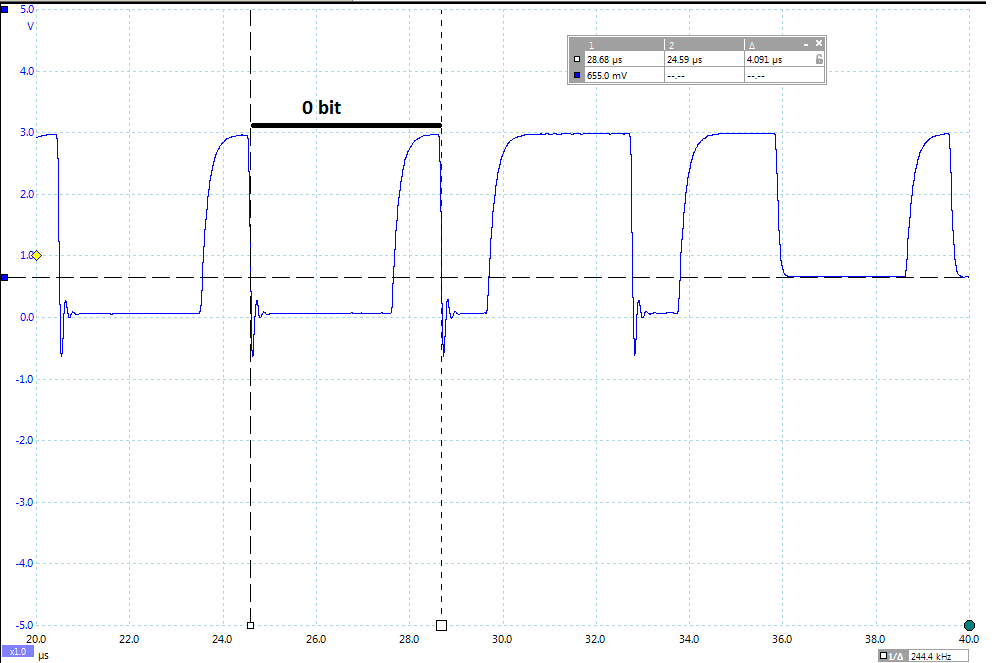
\includegraphics[width=\textwidth]{0bit.png}
\\1 state: the voltage value of the signal is lowered to \SI{0.655}{\V} for \SI1{\us} and
then released to its initial state.
\\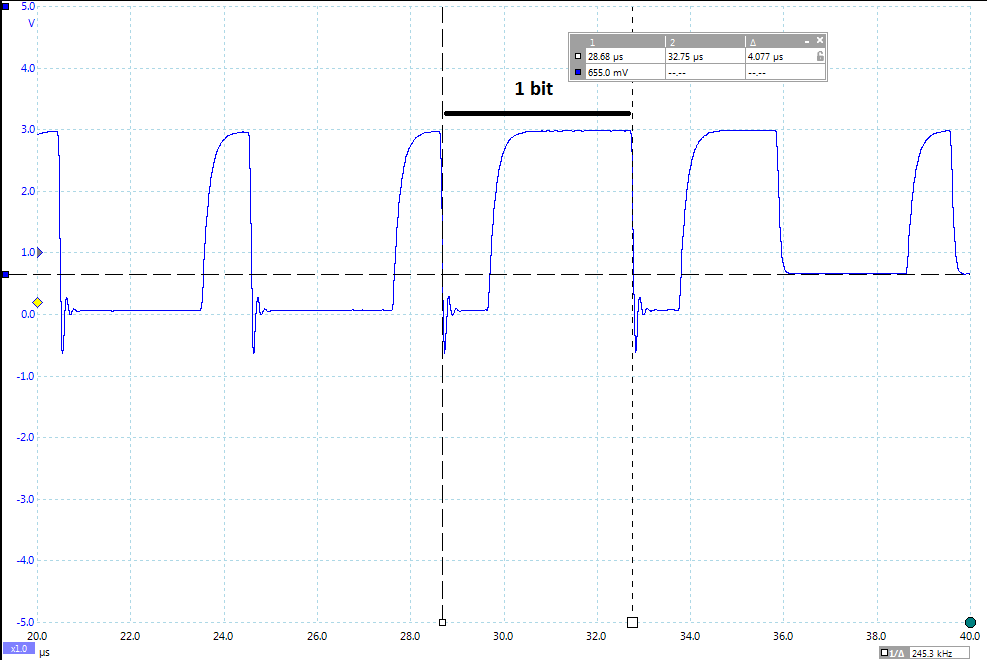
\includegraphics[width=\textwidth]{1bit.png}

Request signal:
The game console requests the inputs from the paddle, which puts the signal in a
certain sequence of 0 and 1 states depending on which buttons are simultaneously
pressed. This request consists of 1 Byte read as follow: 00000001 or 0x01.
N.B. The voltage is lowered to \SI0{\V} during the request sequence, not \SI{0.655}{\V} as
for the inputs signal.

\subsubsection{Inputs signal}
It consists of a 4 Bytes sequence representing the simultaneous inputs of the
paddle buttons and joystick, read as follow:

\begin{itemize}
\item Byte 0:

  \begin{tabular}{|*{8}{C|}}
    \hline
    \multicolumn{1}{|l}{7}&\multicolumn{6}{c}{}&\multicolumn{1}{r|}{0}\\
    \hline
    A&B&Z&Start&DPad up&DPad down&DPad left&DPad right\\
    \hline
  \end{tabular}
\item Byte 1:

  \begin{tabular}{|*{8}{C|}}
    \hline
    \multicolumn{1}{|l}{7}&\multicolumn{6}{c}{}&\multicolumn{1}{r|}{0}\\
    \hline
    Reserved&Reserved&L&R&C up&C down &C left&C right\\
    \hline
  \end{tabular}
\item Byte 2: Joystick X axis range from -128 (left position) to 127 (right
  position)
\item Byte 3: Joystick Y axis range from -128 (down position) to 127 (up position)
\end{itemize}
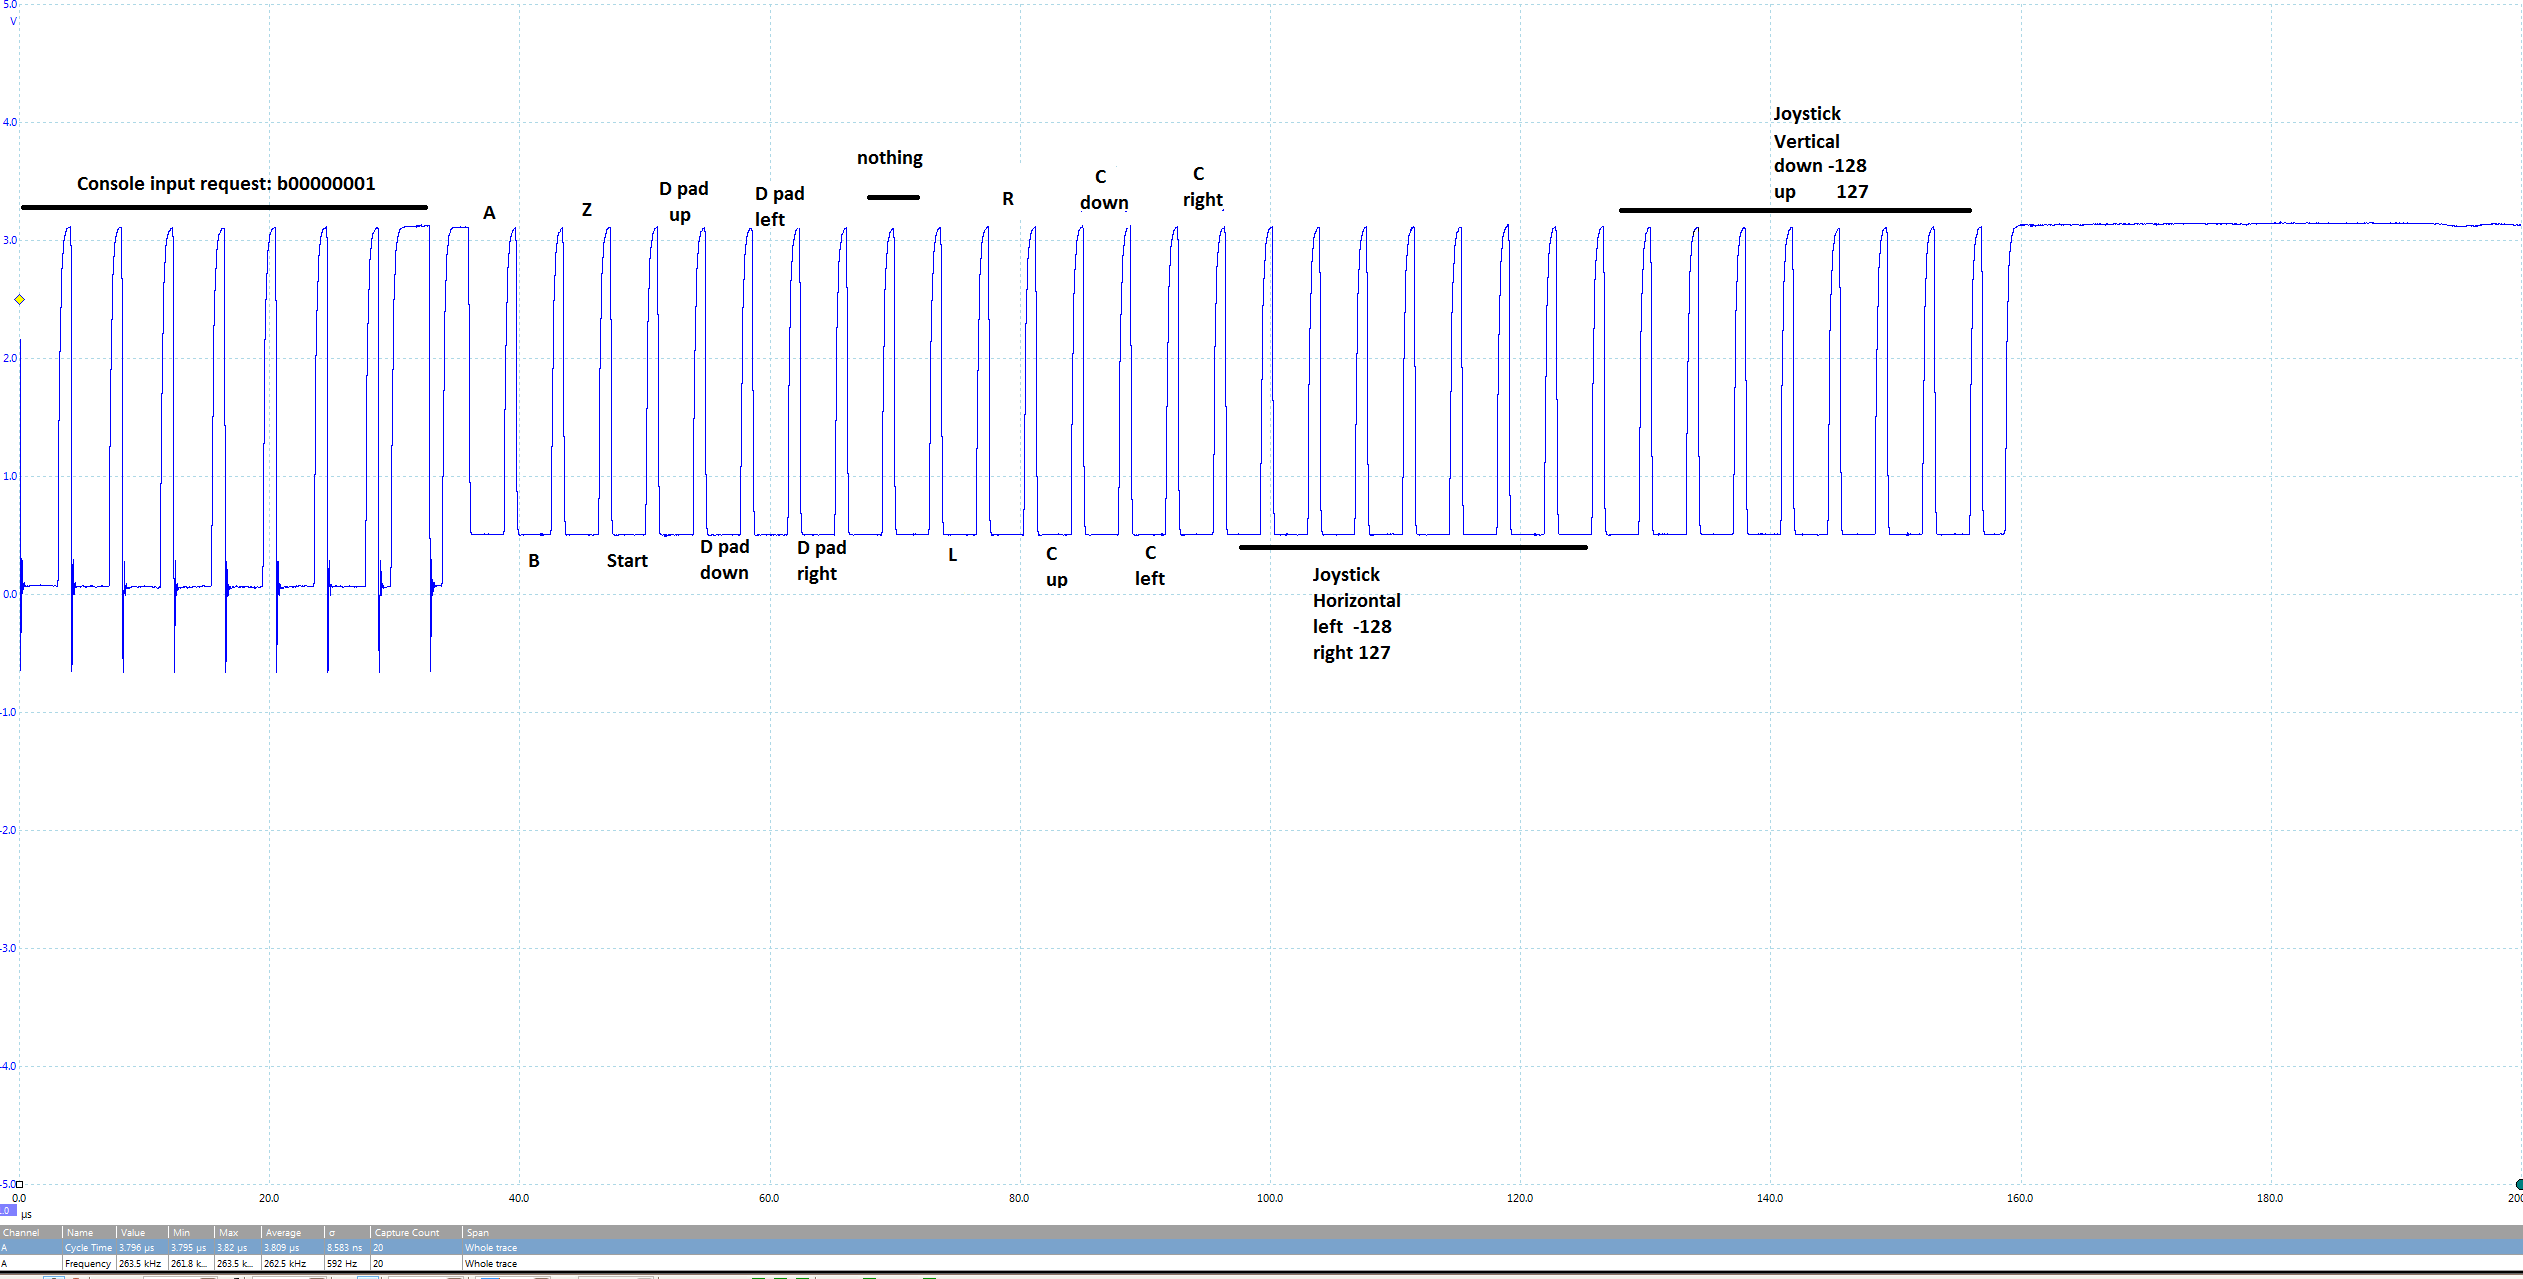
\includegraphics[width=\textwidth]{input_legend.png}
\\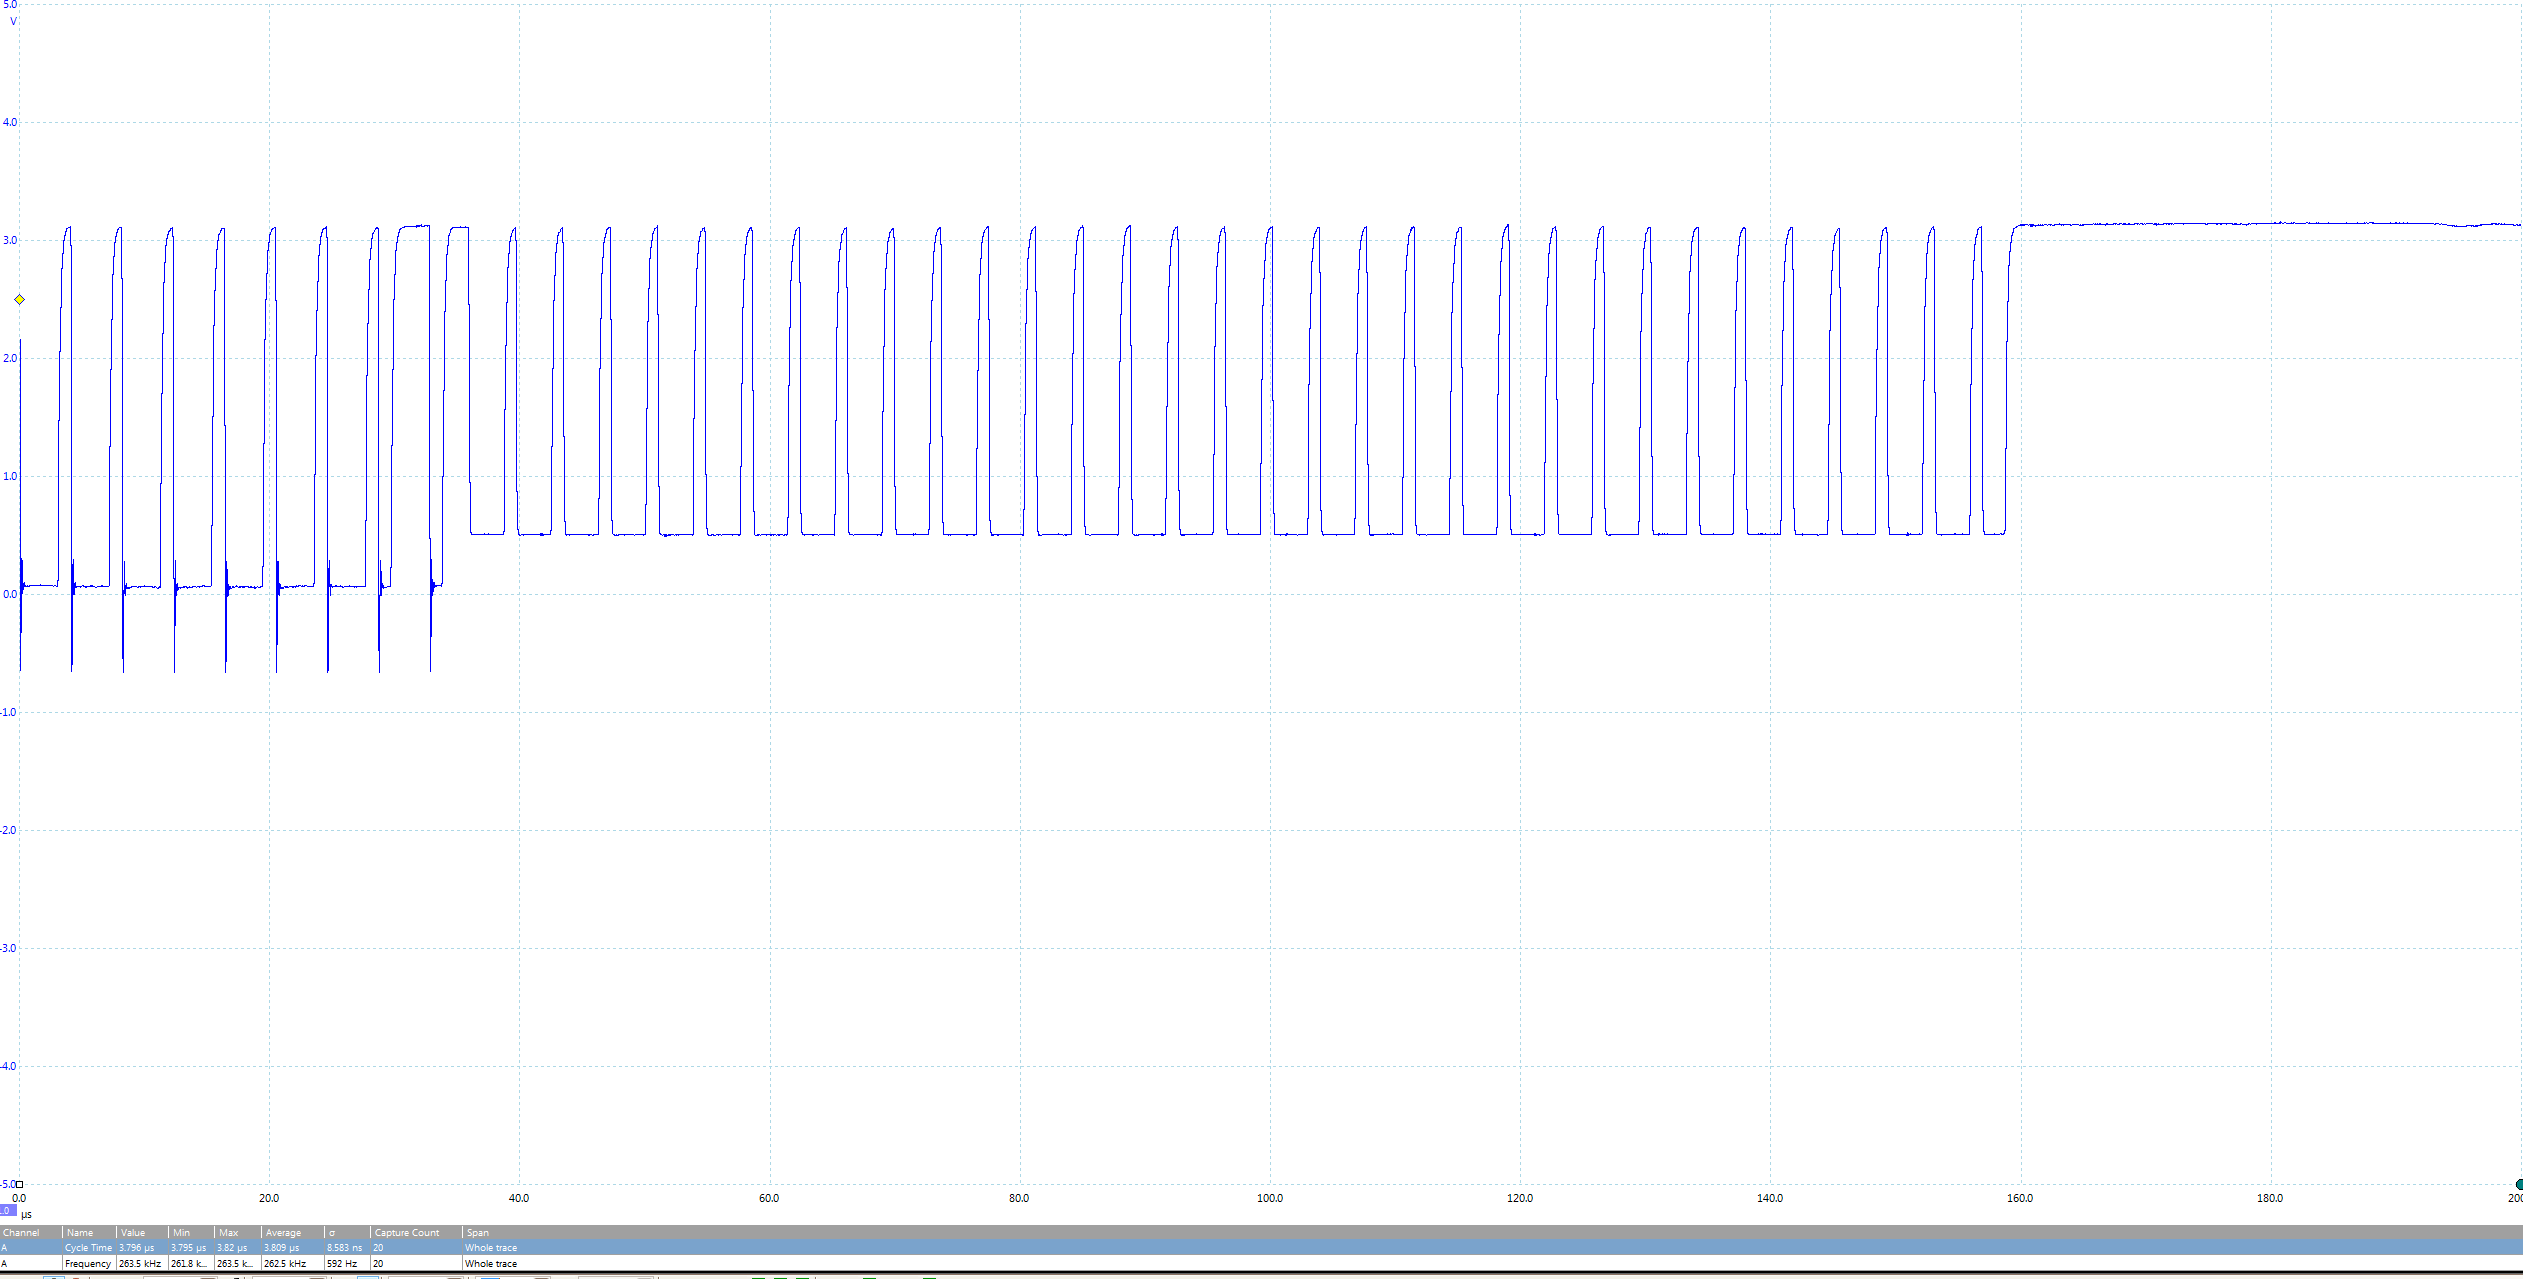
\includegraphics[width=\textwidth]{noinput.png}
\\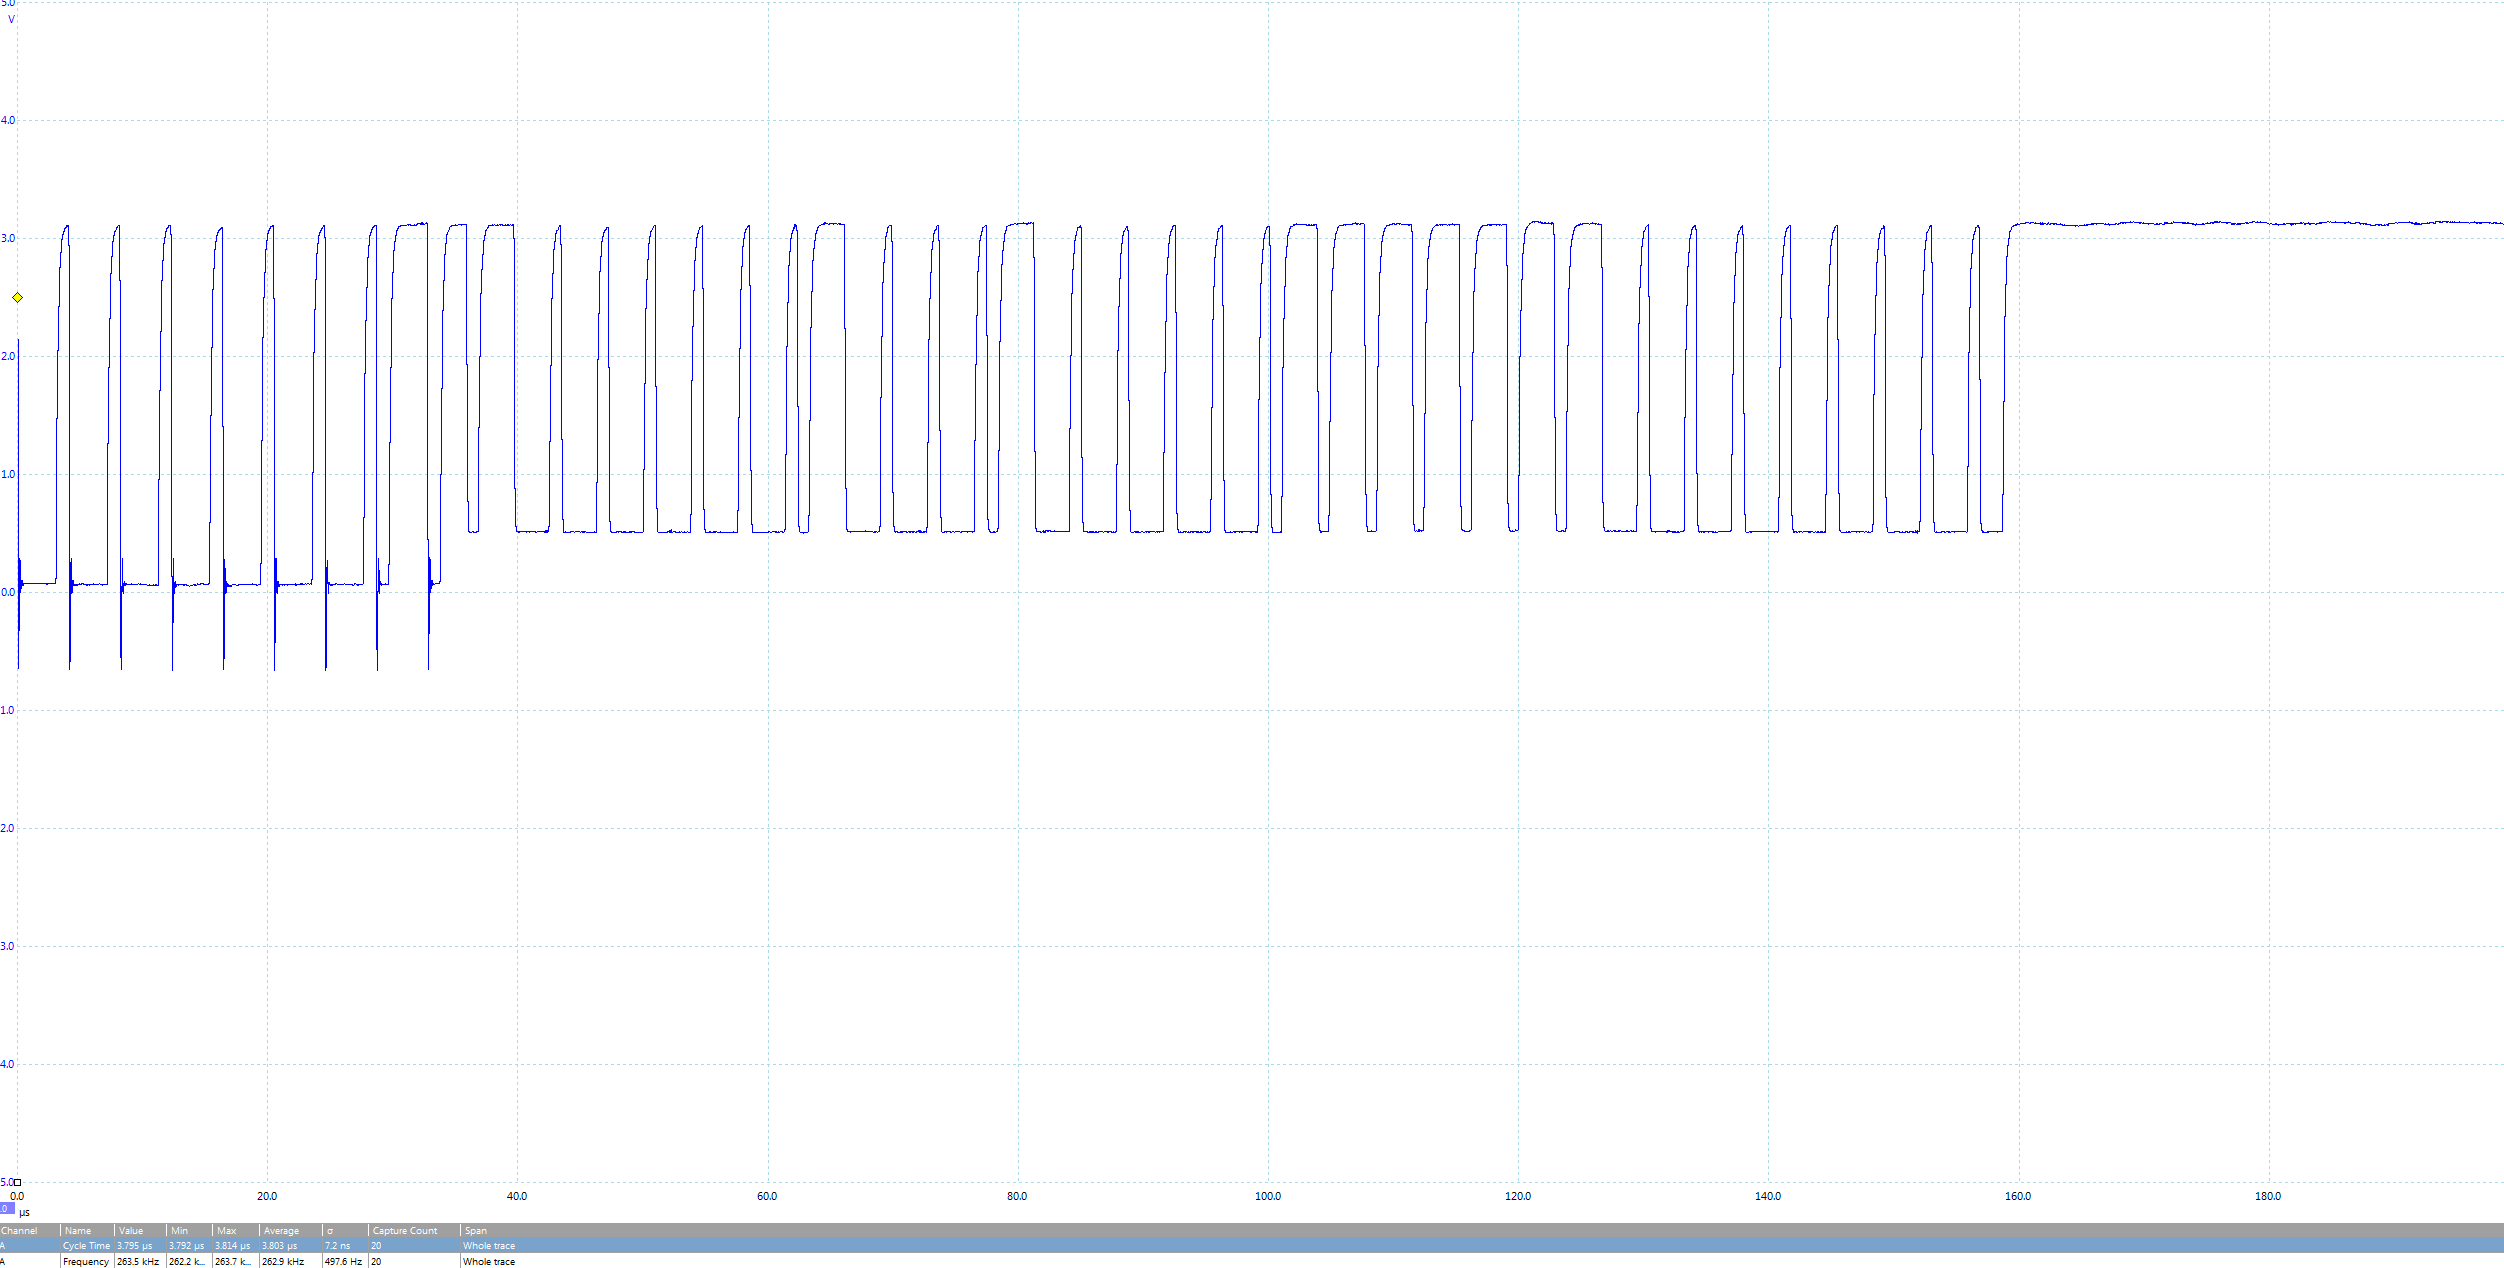
\includegraphics[width=\textwidth]{some_input.png}

\subsection{Mupen64 movie files}

\subsection{SD card}

\subsection{LCD display}

\section{Block diagram}

\section{Preliminary Bill of Materials}
\end{document}